\subsection{Ultrasonic evaluation}
\begin{figure}
    \begin{subfigure}[b]{\picwidth}
        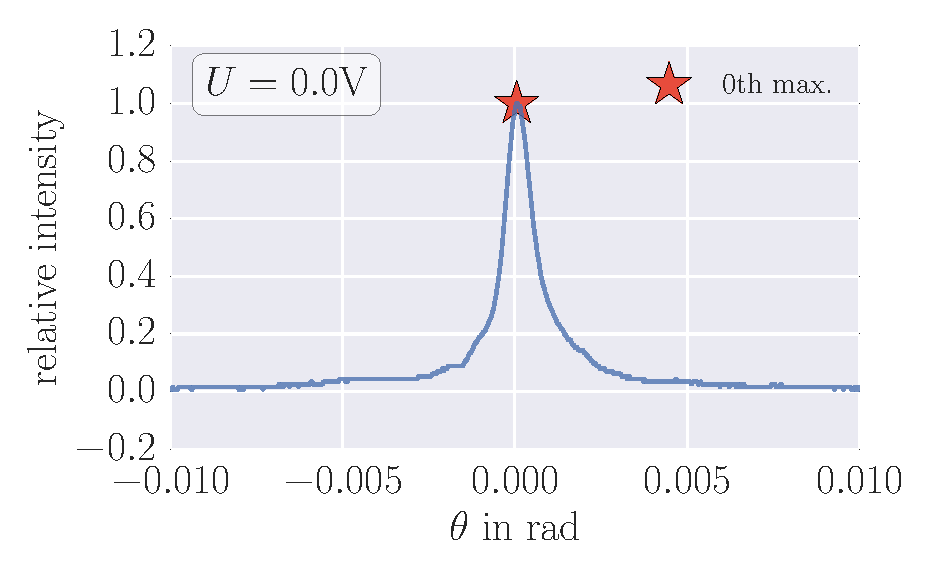
\includegraphics[width=1.2\textwidth]{analysis/figures/raman_001}
        \caption{}
        \label{fig:raman_001}
    \end{subfigure}\qquad
    \begin{subfigure}[b]{\picwidth}
        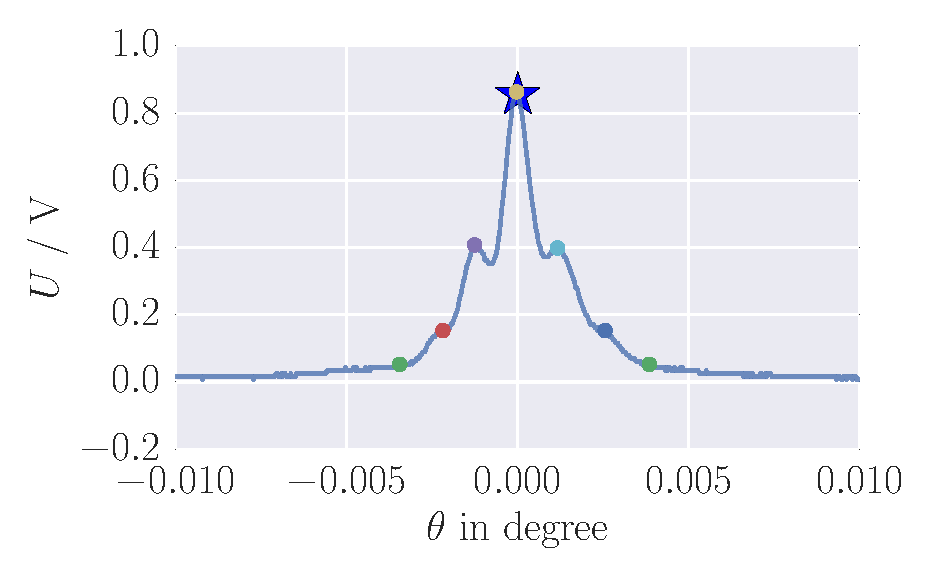
\includegraphics[width=1.2\textwidth]{analysis/figures/raman_007}
        \caption{}
        \label{fig:raman_007}
    \end{subfigure}
    \begin{subfigure}[b]{\picwidth}
        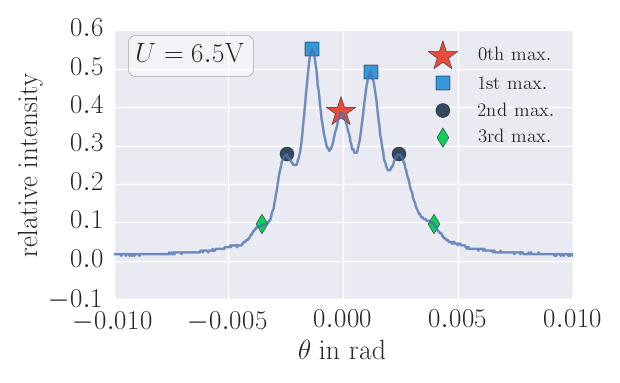
\includegraphics[width=1.2\textwidth]{analysis/figures/raman_014}
        \caption{}
        \label{fig:raman_014}
    \end{subfigure}
    \begin{subfigure}[b]{\picwidth}
        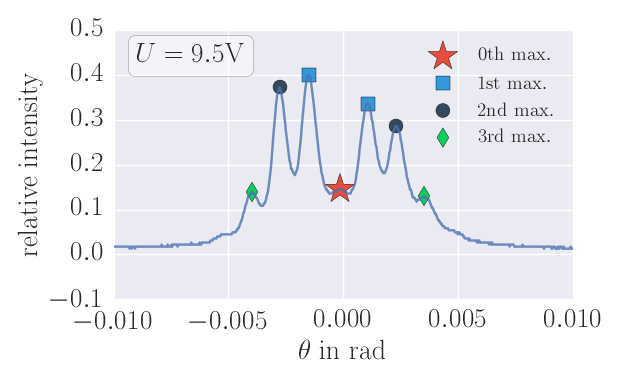
\includegraphics[width=1.2\textwidth]{analysis/figures/raman_020}
        \caption{}
        \label{fig:raman_020}
    \end{subfigure}
    \caption{A subsection of the data from the ultrasonic experiment.}\label{fig:raman}
\end{figure}
\begin{figure}[htpb]
    \centering
    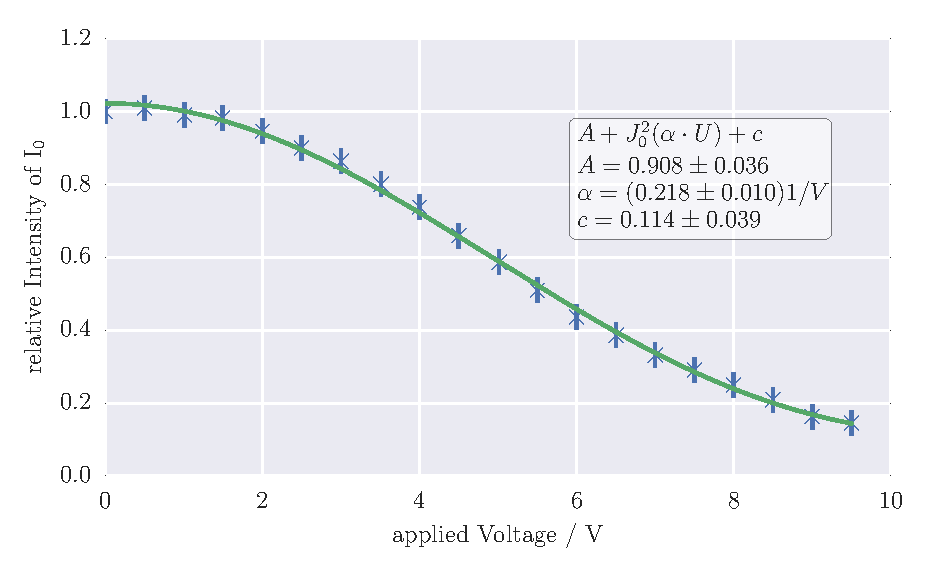
\includegraphics[width=1\textwidth]{analysis/figures/besselfit_0}
    \caption{This is the fit of the maxima of zeroth order. The error is given by 3\% of the extent of the oscilloscope.}
    \label{fig:besselfit_0}
\end{figure}

\begin{table}
    \centering
    \caption{covariance matrix}
 \begin{tabular}{|r|r|r|r|}
 \hline 
\cellcolor[RGB]{204,204,255}&\cellcolor[RGB]{204,204,255}$\alpha$&\cellcolor[RGB]{204,204,240}$A$&\cellcolor[RGB]{204,204,225}$c$\\ \hline 
 \cellcolor[RGB]{204,204,255}$\alpha$&$0.000$ &$-0.000$ &$0.000$ \\ \hline
\cellcolor[RGB]{204,204,240}$A$&$-0.000$ &$0.001$ &$-0.001$ \\ \hline
\cellcolor[RGB]{204,204,225}$c$&$0.000$ &$-0.001$ &$0.002$ \\ \hline
\end{tabular}
\begin{align}
    \Rightarrow \qquad
    \alpha &=& 0.218 \pm 0.010 \\
    A &=& 0.91 \pm 0.04 \\
    c &=& 0.11 \pm 0.04 
\end{align}
\end{table}

